% Drawing 43/03-9 -- folder 43, batch 03, archive page 48 (PDF page 49).
% Transcription: en haut de la colonne de droite, un croquis : à gauche une courte courbe portant un point ; à droite une courbe portant un point, un petit ovale accroché à ce point, et qui traverse plus bas un disque hachuré.
% Kind: two curves with marked points, one crossing a hatched disk. Method 2 (schematic redraw from the facsimile). Status: ok.
% Notes: Ink. Left: a short curve with a marked point. Right: a longer curve from the upper right down to the lower left, a marked point on it with a small upright oval hanging to its right, then a hatched disk which the curve crosses before going on below. The hatching is drawn as horizontal strokes clipped to the disk. Redrawn 2026-11-12 (issue 128): to check again.
% Coordinates: 1 unit = 1 mm = 1/100 of the crop width, y downwards as on the crop (bbox in page fractions: [0.8, 0.06, 0.94, 0.16]).
% Redrawn by Claude (claude-fable-5-2), issue #128, 2026-11-12; not checked by a human; not compiled (no TeX in the session).
% Rights: reproduces part of the work -- behind RENDER_TRANSCRIPTS, never published by itself.
\documentclass[tikz,border=3pt]{standalone}
\usepackage{amsmath,amssymb}
\usetikzlibrary{patterns,arrows.meta}
\tikzset{pencil/.style={black!45}, struck/.style={black!35}, mpt/.style={circle,draw,inner sep=1.3pt}, pt/.style={circle,fill,inner sep=0.9pt}, opt/.style={circle,draw,fill=white,inner sep=1.1pt}, Rd/.style={red!75!black}, Gn/.style={green!45!black}, Br/.style={brown!70!black}}
\begin{document}
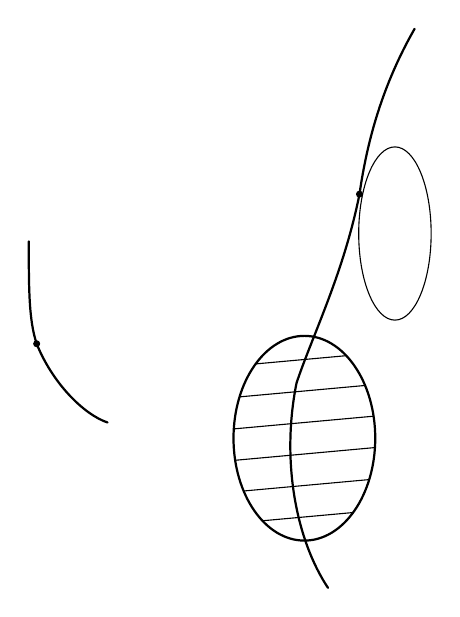
\begin{tikzpicture}[x=1mm,y=-1mm,line cap=round,line join=round,font=\small]
\draw[thick] (30,44) .. controls (30,50) and (30,54) .. (31,57) .. controls (33,62) and (37,66) .. (40,67);
\node[pt] at (31,57) {};
\draw[thick] (79,17) .. controls (75,24) and (73,31) .. (72,38) .. controls (70,48) and (66,56) .. (64,62) .. controls (62,72) and (64,82) .. (68,88);
\node[pt] at (72,38) {};
\draw (76.5,43) ellipse [x radius=4.6, y radius=11];
\draw[thick] (65,69) ellipse [x radius=9, y radius=13];
\begin{scope}
\clip (65,69) ellipse [x radius=9, y radius=13];
\foreach \y in {59,63,...,81} {
\draw (54,\y+1) -- (76,\y-1);
}
\end{scope}
\end{tikzpicture}
\end{document}
